\section{Net Helper}
In this section are explained specific problematiques and solutions for implementing \textit{net-helper} in
\textbf{TCP}.

\subsection{Nethelper: UDP vs TCP}
Considering the programming logics on implementing the nethelper as defined in the previous section, the two
main differences are:
\begin{itemize}
  \item \textit{Multiple connections}: in \textbf{TCP} each node correspond to a different socket descriptor,
    whereas in \textbf{UDP} there is a single socket which is used for retriving data.
  \item \textit{message size}: in \textbf{UDP} the data are sent without any attention on size of
    sent data, whereas in \textbf{TCP} such controls are intrinsically embedded. 
\end{itemize}
More detalis are reported in following subsections.

\subsection{Multiple Connections issue}
This is a problem deriving from the logics on which is based \textbf{TCP}. It uses a mapping between a node
and the corresponding socket descriptor. This does not have any consequences on sending process, whereas there
is some at the receiving one. Some difficulties on overcomming this problem arised due to the fact that the
interface used by \textit{net-helper} was defined at the very beggining phase of design \textbf{GRAPES}
library. The protocol planned to be used at that moment was \textbf{UDP}, thus some more general issues
were not taken in consideration. In particular, this is related to the fact that the \textit{net-helper}'s
interface only provides a data-structure \textit{nodeID} which represents the node itself. For this reason,
within such structure are embedded some extra tools such managing the known neighbours.

\subsubsection{solution}
As mentioned before, all neighbours are collected and stored into a \textit{nodeID} data structure that
is the node itself.
\begin{lstlisting}
typedef struct {
    dict_t neighbors;
    int srvfd;
    aqueue_t aqueue;
} local_t;

typedef struct nodeID {
    unsigned refcount;
    sockaddr_t addr;
    local_t *loc;
} nodeid_t;
\end{lstlisting}

These structures are used in particular at sending and at receiving phases:
\begin{lstlisting}
int send_to_peer(const struct nodeID *self, struct nodeID *to,
                 const uint8_t *buffer_ptr, int buffer_size)
\end{lstlisting}
\paragraph{Sending phase}: the interface provides two \textit{nodeID} data-structure: \textit{self} and
\textit{to} that correspond to the sender and receiver, respectively. In both cases, there is a local
data-structure that provides tools for managing the neighbours such as a dictionary hash-mapp. The later
one, uses  the sock-addresses of the neighbours as keys for the mapping. This permitts to select the target
node.

\begin{lstlisting}
int recv_from_peer(const struct nodeID *self, struct nodeID **remote,
                   uint8_t *buffer_ptr, int buffer_size)
\end{lstlisting}
\paragraph{Receiving}: in this case, the \textit{self-nodeID} data-structure is of much more interest
considering that it scans the incoming messages, without any particular attention to their sender.


\subsection{Message size issue}
Another problem reguarding \textbf{TCP} is the fact it has to manage messages' size and completness.
\textbf{UDP} does not take in account such problem considering that it sends the data in burst without
worrying about the size. The advantage of such behaviour is that there is a reduced delay considerig that
the protocol does not execute any control the transmitted data. This is optimal for its usage in real-time
applications, whereas at receiving side, \textbf{TCP} needs to wait for a complete transittion or hold on
partial data transmittion.

\subsubsection{solution}
The operations reguarding the sending and receiving are modeled as state-machine processes.

\begin{figure}[ht!]
  \begin{center}
    \subfigure[Sender's]{%
      \label{fig:first}
      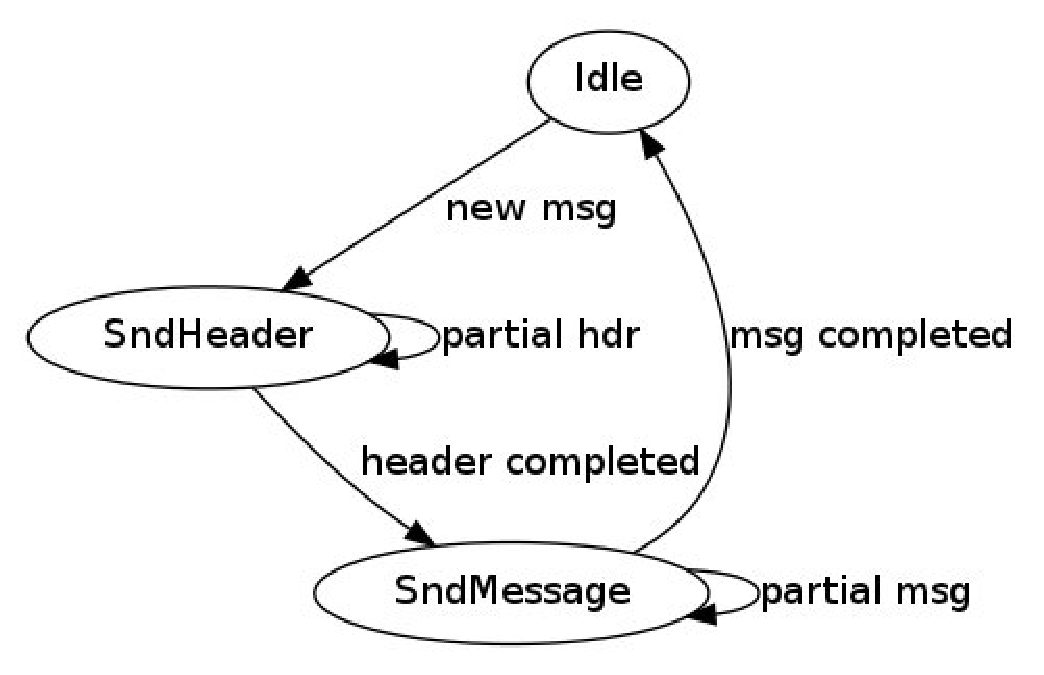
\includegraphics[width=0.6\textwidth]{figures/sender}
    }%
    \subfigure[Receiver's]{%
      \label{fig:second}
      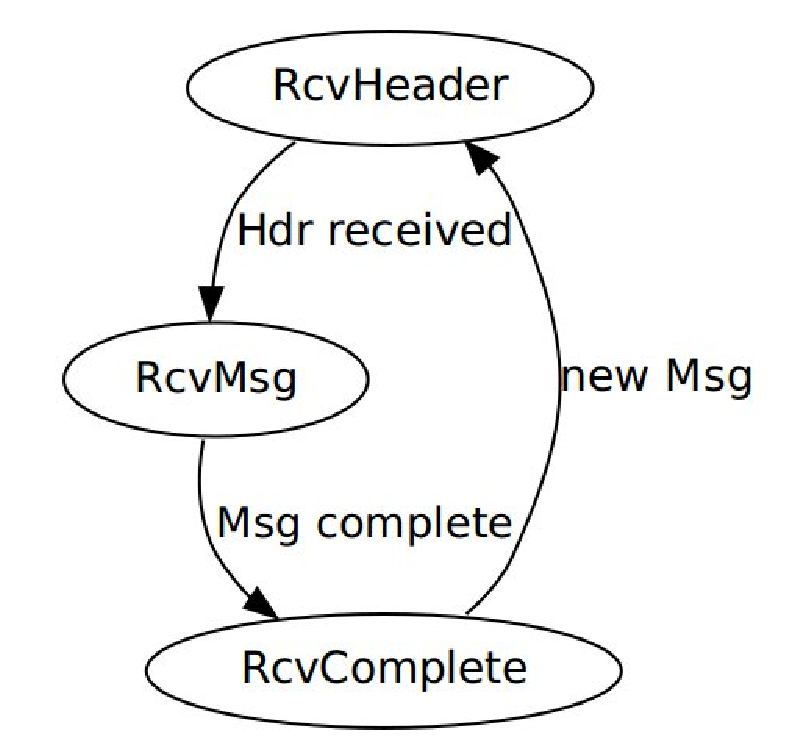
\includegraphics[width=0.5\textwidth]{figures/receiver}
    }%
  \end{center}
  \caption{%
    State Machines
  }%
\end{figure}
\paragraph{Sender}:
\paragraph{Receiver}:
